\chapter{Megvalósítás}
\section{Alkalmazott módszerek}
A megvalósítás során az eddig megismert módszereket fogom felhasználni, azokat Python programozási nyelven fogom elkészíteni és ismertetni. Az egyes algoritmusokat függvények formájában készítem el, ezeket a függvényeket pedig több Python szkriptben is felhasználom.
\par Az eddig megismert módszerek közül elsősorban a nyers bemenetből emelem ki a játékterületet, ezt követően a golyók pozíciójának felismeréséhez kör detektálást és egy neurális hálózatot fogok használni. A neurális hálózat betanításához az adatkészletet kör detektálással, mintaillesztéssel és kézi válogatással fogom elkészíteni. A következőkben az egyes függvények működését, azokban felhasznált külső könyvtárak eszközeit ismertetem részleteiben.
\par A fejezetek felosztása az eddig megismert lépések szerint kerül rendezésre.

\section{A golyók pozíciója}

\subsection{A szükséges könyvtárak importálása}
Ahhoz hogy a függvények megfeleően működjenek, meg kell mondanunk a programnak, hogy használja a külső könyvtárakat.
\newline Ezt a következőképp tehetjük meg.

\vspace{2mm}\begin{lstlisting}[language=Python, numbers=left]
import math
import numpy as np
import cv2
\end{lstlisting}

\par A \lstinline{math} könyvtár segítségével matematikai műveleteket (gyökvonás, szinusz, koszinusz) tudunk végezni, a \lstinline{numpy} könyvtár a tömbök, mátrixok kezelését, azokkal való műveleteket segíti és gyorsítja, a \lstinline{cv2} pedig az OpenCV eszközeit teszi elérhetővé.

\subsection{Az asztal kontúrjának megkeresése}
Annak érdekében, hogy a nyers képből kinyerjük a játékterületet, azt először be kell tölteni egy többdimenziós tömbbe. A kép betöltése többféleképp végbemehet, ezért ezt konkrétan nem részletezem.
\par A betöltött kép tömbjének alakja megegyezik a kép szélességével és magasságával, továbbá az intenzitási értékekkel, tehát ha betöltünk egy 1024 x 512 méretű RGB képet, annak tömbjének az első és második dimenziója 1024 és 512, a harmadik pedig az RGB (Piros, Zöld, Kék) intenzitásoknak megfelelően 3 méretű.
\par Fontos megjegyezni, hogy az OpenCV a képeket betöltéskor BGR formátumban tölti be, ez az elnevezésből adódóan annyiban tér el az RGB formátumtól, hogy a piros (R) és kék (B) színcsatornák fel vannak cserélve.
\par A nyers bemeneti kép megszerzése után készen állunk az asztal kontúrjának megkeresésére. Első lépésként a képet átalakítjuk HSV formátumra, majd megadjuk az alsó és felső intenzitási értékhatárokat, amelyből elkészítjük a maszkot. Ezután maszkoljuk az eredeti képet a maszk segítségével.
\newline Ezt a következő kódsorokkal végezhetjük el.


\vspace{2mm}\begin{lstlisting}[language=Python, numbers=left]
hsv = cv2.cvtColor(image, cv2.COLOR_BGR2HSV)

lower_green = np.array([40, 190, 50])
upper_green = np.array([65, 255, 225])

mask = cv2.inRange(hsv, lower_green, upper_green)

result = cv2.bitwise_and(image, image, mask = mask)
\end{lstlisting}

\par A kódban az \lstinline{image} a bemeneti képünk, amelyet a \lstinline{cv2.cvtColor} függvénnyel \cite{cv2_cvt_color} konvertálunk át HSV formátumra. Ennek a függvénynek az első paramétere a bemeneti képünk, a második pedig a konverzió típusa, amely ebben az esetben BGR $\rightarrow$ HSV. A \lstinline{lower_green} és \lstinline{upper_green} változók az alsó és felső intenzitási határokat jelölik sorrendnek megfelelően. A maszk elkészítését a \lstinline{cv2.inRange} függvénnyel \cite{cv2_in_range} végezhetjük el itt a paraméterek sorban a HSV re konvertált képünk, valamint az alsó és felső intenzitás értékek.
\newline A függvény a következők alapján dönti el, a maszk intenzitását,

\begin{equation}
    M(I) = L(I) \le S(I) \le U(I)
    \label{for:maszkolas}
\end{equation}

\par ahol $M$ a maszk, $L$ az alsó, $U$ a felső és $S$ a bemeneti HSV képet jelöli. A \ref{for:maszkolas} függvény mindhárom intenzitásra alkalmazásra kerül, a maszkban az intervallumon belüli intenzitások 255, a kívüliek pedig 0 értéket kapnak. A maszk elkészítése után azt alkalmazzuk az eredeti bemenő képre a \lstinline{cv2.bitwise_and} függvény \cite{cv2_bitwise_and} segítségével. Itt a paraméterek a bejövő eredeti kép \lstinline{image} kétszer és a maszk \lstinline{mask}.
\newline A folyamat során a metódus a következőképp jár el,

\begin{equation}
    R(I) = S_1(I)\quad \land\quad S_2(I)\qquad ,ha\quad M(I) \ne 0
    \label{for:maszk_alkalmazas}
\end{equation}

\par ahol $R$ a kimenő maszkolt kép (\lstinline{result}) $S_1$ és $S_2$ a két bemeneti kép paraméter, és $M$ a maszk. A bemenetben a kép azért szerepel kétszer egymás után, mert a \ref{for:maszk_alkalmazas} függvényben láthatóan a két bemenő paraméter közt egy bit szintű 'és' művelet történik, amennyiben a maszk nem nulla. Ez azt teszi lehetővé, hogy az eredeti képet kapjuk a maszkolt elemek kivételével, ami azért történik, mert bit szinten ha két megegyező elem közt történik 'és' művelet, akkor az eredmény szintén megegyezik a két elemmel. Ennek a folyamatnak a kimenetele látható a már előzőleg tárgyalt \ref{fig:bemeneti_kep_mask} ábrán.
\par A maszkolt kép megszerzése után elvégezhetjük az éldetektálást, amelyet megelőz egy szürkeárnyalatolás.
\newline Ezeket a műveleteket a következő programsorokkal végezhetjük.

\vspace{2mm}\begin{lstlisting}[language=Python, numbers=left]
image_gray = cv2.cvtColor(result, cv2.COLOR_BGR2GRAY)

edges = cv2.Canny(image_gray, 100, 200)
\end{lstlisting}

\par A szürkeárnyalati konverziót a már megismert \lstinline{cv2.cvtColor} függvénnyel \cite{cv2_cvt_color} végezzük el, majd ezután megkeressük az éleket a képen Canny éldetektálás \cite{cv2_canny,canny_edge_detection} (\lstinline{cv2.Canny}) segítségével.
\newline A Canny éldetektálás általában több lépésre bontható szét, ezek lehetnek:

\begin{itemize}
    \setlength\itemsep{-2pt}
    \item Homályosítás Gauss szűrővel \cite{shapiro2001} a zajcsökkentés érdekében
    \item Élek helyének és irányának megállapítása intenzitás-gradiensből
    \item Nem-Maximum vágás merőleges élek szűréshéhez
    \item Kettős küszöbölés élek szűréséhez
\end{itemize}

\par Az éldetektálásnál meg kell adnunk a függvénynek a szürkeárnyalatos képünket (\lstinline{image_gray}), továbbá két küszöbértéket, amelyet a Canny detektálás a kettős küszöbölés folyamat során fog felhasználni. Itt, ha a felső küszöb felett van egy potenciális él, azt felvesszük az élek közé, ha az alsó küszöb alatt van eldobjuk és ha a felső és alsó küszöbök közt helyezkedik el, akkor a szomszédos pixelek alapján vesszük fel élnek. Az éldetektálással kapott kép (\lstinline{edges}) a \ref{fig:bemeneti_kep_edge} ábrán látható.

\begin{figure}[!ht]
    \centering
    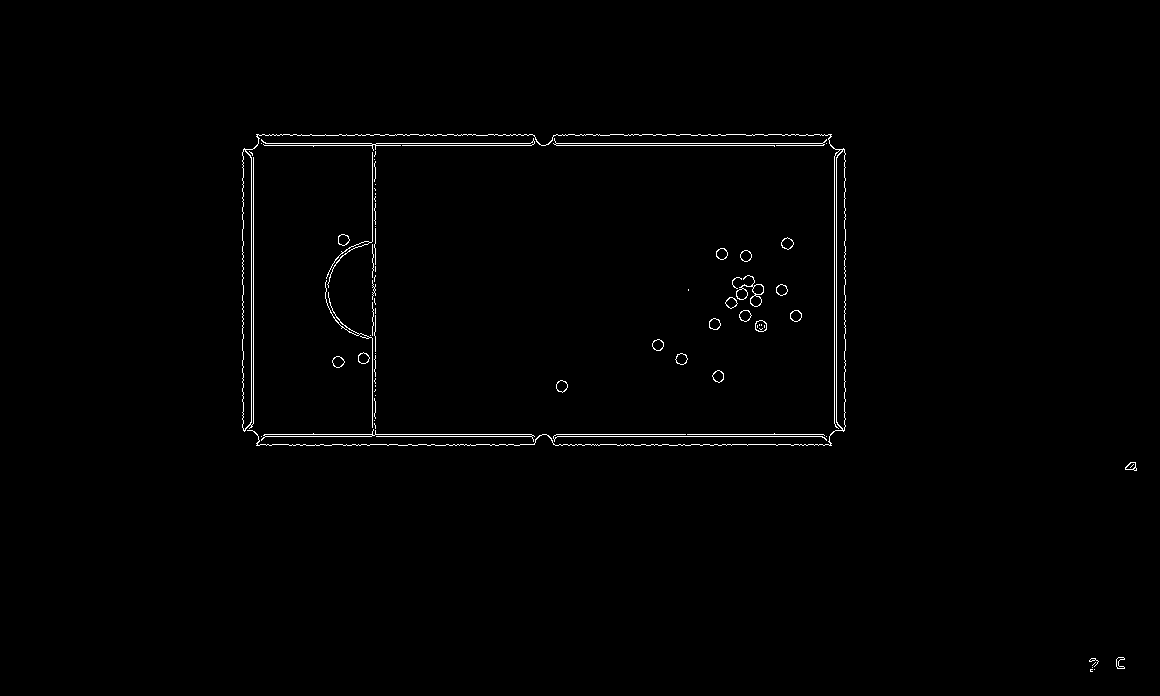
\includegraphics[width=150mm, keepaspectratio]{figures/input_screen_edge.png}
    \caption{A Canny éldetektálás után kapott kép.}
    \label{fig:bemeneti_kep_edge}
\end{figure}

\par A következő lépésben a bináris képen lefuttatásra kerül egy kontúrkereső algoritmus \cite{SUZUKI198532}, majd a kapott kontúroknak vesszük a konvex körvonalát, azok egyszerűsítése, esetleges konkáv alakzatok megszüntetése érdekében. Ezek után feltételezve, hogy a kontúrok közül a legnagyobb a játékterület, kiválasszuk a körvonalak közül.
\newline Az említett folyamatokat a következő függvényekkel hajtom végre,

\vspace{2mm}\begin{lstlisting}[language=Python, numbers=left]
contours, _ = cv2.findContours(edges, cv2.RETR_LIST, cv2.CHAIN_APPROX_SIMPLE)

contours = [cv2.convexHull(c) for c in contours]
contours = sorted(contours, key=lambda x : cv2.contourArea(x), reverse=True)[:1]
\end{lstlisting}

\par A \lstinline{cv2.findContours} függvény \cite{cv2_find_contours, SUZUKI198532} egy határkövetéses algoritmussal kigyűjti a kontúrokat. Ezek a kontúrok a képen található képpont koordináták láncolatából állnak össze. A kontúrok körvonalát a \lstinline{cv2.convexHull} függvény \cite{cv2_convex_hull,SKLANSKY198279} segítségével kapjuk meg. Ez az algoritmus a kontúrok koordinátáinak láncolatát használja, majd a kontúrt egy konvex körvonallal határolja, ugyancsak koordináták láncolatai formájában reprezentálva.
\par A fenti művelet elsőre feleslegesnek tűnhet, hiszen a keresett asztal kontúrja előreláthatólag nem konkáv, a művelet elvégzése mégis fontos, hiszen így egyszerűsíthetjük az alakzatunkat (pl.: kotúr koordináta láncolat pontjainak csökkentése), ezzel a következő műveleteket felgyorsítva.
\par A legnagyobb kontúr kiválasztásához tudnunk kell az egyes kontúrok területét. A területet a \lstinline{cv2.contourArea} függvénnyel \cite{cv2_contour_area} számolhatjuk ki. Ezt megtesszük minden eddigi kontúrral úgy, hogy szimplán paraméterként adjuk a függvénynek. A kiszámolt területek közül kiválasszuk a legnagyobbat, majd annak kontúr koordináta láncolatát eltároljuk. A kapott kontúr kirajzolva a \ref{fig:bemeneti_kep_contour} ábrán látható.

\begin{figure}[!ht]
    \centering
    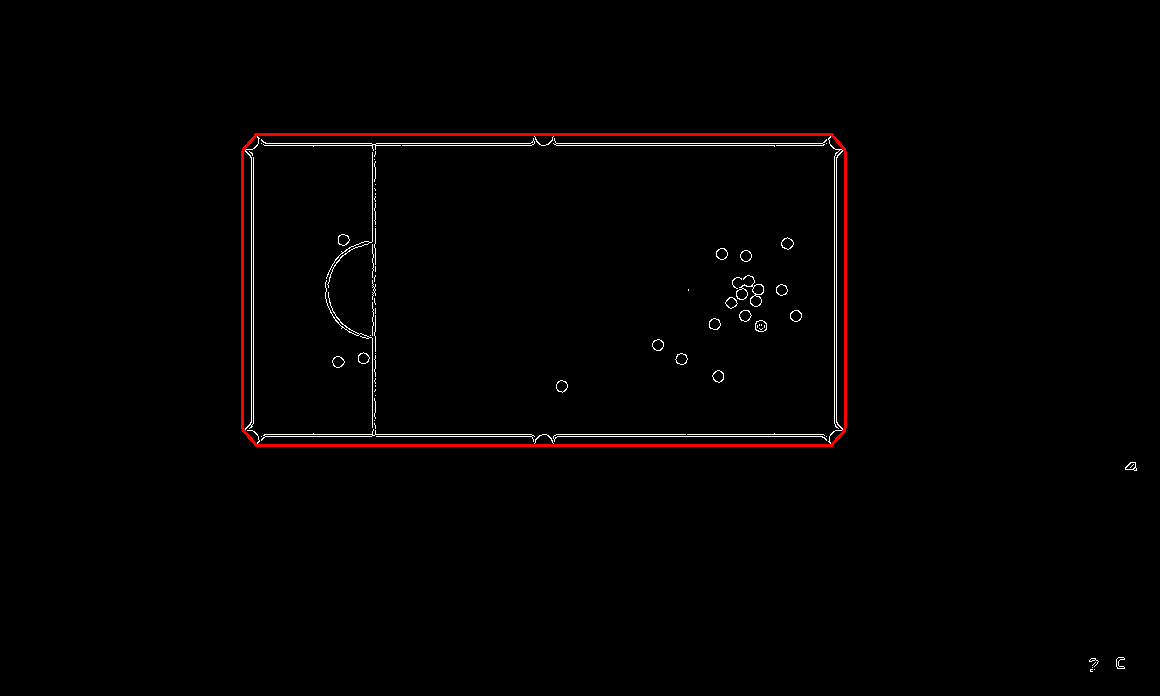
\includegraphics[width=150mm, keepaspectratio]{figures/input_screen_contour.png}
    \caption{A felismert asztal kontúrja a bináris képen, piros körvonallal keretezve.}
    \label{fig:bemeneti_kep_contour}
\end{figure}

\par A \lstinline{cv2.contourArea} függvény a Surveyor's Area algoritmust \cite{braden1986surveyor} használja az alakzatok területének számolásához. Ez az algoritmus a Green-tétel egy speciális esete, amely alkalmazható egyszerű sokszögekre.
\newline Az algoritmus függvéyne a következő,

\begin{equation}
    A = \sum^n_{k=0}\frac{(x_{k+1} + x_k)(y_{k+1} - y_k)}{2}
    \label{for:green_formula}
\end{equation}

\par ahol $n$ az óramutató járásával ellentétesen rendezett kontúr koordináták száma, $(x_k, y_k)$ a $k$ adik koordináta $x$ és $y$ pozíciója, és feltételezhetjük, hogy a $k = n+1$ elem megegyezik a $k = 0$ elemmel.

\par A \ref{fig:bemeneti_kep_contour} ábrán látható, hogy a kontúrunk téglalaphoz hasonló alajkának ellenére több, mint 4 pontból áll. Ahhoz hogy téglalap formájában ki tudjuk vágni a képet, meg kell keresnünk azt a négyszöget, amely a kontúrt határolja. Erre egy olyan algoritmust készítettem, amely megkeresi a kontúr koordináták segítségével a négy leghosszabb oldalt, majd kiszámolja ezek metszéspontját. A négy leghosszabb oldal használata feltételezi, hogy a kép közel felső nézetből készült az asztalró, továbbá, hogy a sarkoknál jelenik meg több pont a kontúr keresés után.
\par Az oldalhosszok számolása a \ref{for:vector_distance} képlet alapján megy végbe,

\begin{equation}
    D = \sqrt{(x_a-x_b)^2 + (y_a-y_b)^2}
    \label{for:vector_distance}
\end{equation}

\par ahol $D$ a kiszámolt pontok közti távolság, $(x_a,y_a)$ és $(x_b,y_b)$ pedig a két koordináta, ameyek közt a távot számoljuk. Miután megkaptuk az oldalak hosszait, kiválasszuk a négy legnagyobbat, majd az ezekhez tartozó koordinátákat tároljuk. A kiválasztott pontokat fontos, hogy óramutató járásával ellentétes sorrendben rendezzük, amennyiben nem a négyszög kontúrunk később hibás lehet.
\par A metszéspontok kiszámolásához a következő képleteket \cite{line_line} használtam,

\begin{equation}
    D = (x_1 - x_2)(y_3 - y_4) - (y_1 - y_2)(x_3 - x_4)
    \label{for:vector_intersection_denominator}
\end{equation}
\begin{equation}
    P_x = \frac{(x_1y_2 - y_1x_2)(x_3 - x_4) - (x_3y_4 - y_3x_4)(x_1 - x_2)}{D}
    \label{for:vector_intersection_point_x}
\end{equation}
\begin{equation}
    P_y = \frac{(x_1y_2 - y_1x_2)(y_3 - y_4) - (x_3y_4 - y_3x_4)(y_1 - y_2)}{D}
    \label{for:vector_intersection_point_y}
\end{equation}

\par ahol a \ref{for:vector_intersection_denominator} képletben a $D$ a \ref{for:vector_intersection_point_x} és \ref{for:vector_intersection_point_y} képletekben a nevező kiszámolásához biztosít könnyebb átláthatóságot, $(P_x, P_y)$ a kiszámolt metszéspont, $(x_1, y_1)$, $(x_2, y_2)$, $(x_3, y_3)$ és $(x_4, y_4)$ pedig a négy pont, amelyek a két egyenest határozzák meg, itt ezek közül az eső kettő az egyik, a második kettő a másik egyeneshez tartozik.
\par A fenti egyenletek kódban a következőképp reprezentálhatóak,

\vspace{2mm}\begin{lstlisting}[language=Python, numbers=left]
def intersection(p1, p2, p3, p4):
 d = (p1[0] - p2[0]) * (p3[1] - p4[1]) - (p1[1] - p2[1]) * (p3[0] - p4[0])
 if (abs(d) < 1e-8):
    return False

 t1 = (p1[0]*p2[1] - p1[1]*p2[0]) * (p3[0] - p4[0]) - (p3[0]*p4[1] - p3[1]*p4[0]) * (p1[0] - p2[0])
 t2 = (p1[0]*p2[1] - p1[1]*p2[0]) * (p3[1] - p4[1]) - (p3[0]*p4[1] - p3[1]*p4[0]) * (p1[1] - p2[1])
 return [t1 / d, t2 / d]
\end{lstlisting}

\par ahol \lstinline{p1}, \lstinline{p2}, \lstinline{p3}, \lstinline{p4} a fent megismert négy koordináta, \lstinline{d} a kiszámolt nevező, \lstinline{t1} és \lstinline{t2} pedig segédváltozók a számlálók tárolásához. A kódrészlet 3. és 4. sorában látható, hogy abban az esetben ha \lstinline{d} nagyon kicsi, a függvény \lstinline{False} értéket ad vissza. Ez azért van, mert a \ref{for:vector_intersection_denominator} függvényben kiszámolt nevező, $D = 0$ esetén a két egyenes párhuzamos.
\par A folyamat végeredményeképp kapott kép a \ref{fig:bemeneti_kep_quad} ábrán látható.

\begin{figure}[!ht]
    \centering
    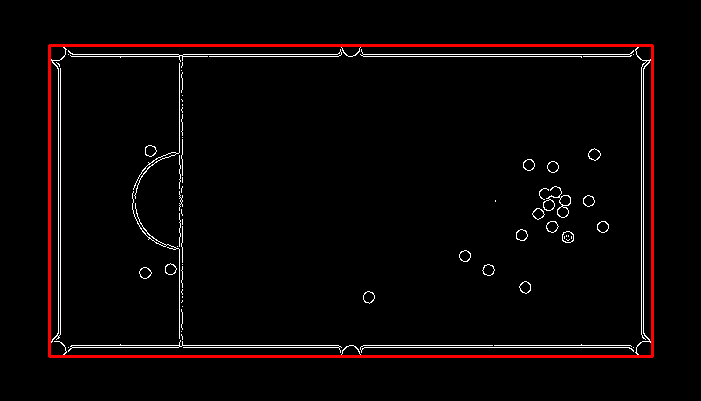
\includegraphics[width=150mm, keepaspectratio]{figures/input_screen_quad.png}
    \caption{A felismert asztal négy pontból álló körvonala a bináris képen, piros körvonallal keretezve.}
    \label{fig:bemeneti_kep_quad}
\end{figure}

\subsection{Az asztal kivágása és torzítása}